\documentclass[10pt]{beamer}
\usetheme{Frankfurt}
\usepackage[utf8]{inputenc}
\usepackage[spanish]{babel}
\usepackage{amsmath}
\usepackage{amsfonts}
\usepackage{amssymb}
\usepackage{graphicx}
\graphicspath{{imagenes/}}									% Ruta de las imagenes, solo escribir nombre de la imagen
\author{Ciro Fabián Bermúdez Márquez}
\title{Síntesis de integradores de orden fraccionario usando hardware analógico reprogramable y sus aplicaciones}
%\setbeamercovered{transparent} 
%\setbeamertemplate{navigation symbols}{} 
%\logo{} 
\institute{Benemérita Universidad Autónoma de Puebla} \date{6 de Febrero de 2020} 
%\subject{}

%---------------------------------------------------------------------
%                      Paquetes adicionales                          %
%---------------------------------------------------------------------
%-------------------------------------------------------------------------------
%                                Paquetes extras                               %
%-------------------------------------------------------------------------------

\usepackage{layout}	
\usepackage{xfp}												% Hacer evaluaciones \fpeval{}					
\newcommand\x{470}												% Declaracion de variables
\newcommand\y{700}
\newcommand\cuadro{\fpeval{\x /20}}
% Letterpaper			794 x 614pt		216 x 279mm
%						\textwidth = 500pt
%						\textheight = 681pt

% a4paper				845 x 597pt		297 x 210mm
%						\textwidth = 483pt
%						\textheight = 731pt

\usepackage{lipsum}												% Texto de ejemplo \lipsum[1-30]
\decimalpoint													% Punto decimal en lugar de coma
\spanishsignitems												% Viñetas en lugar de cuadros
\raggedbottom													% Eliminar molestos warnings

\usepackage{comment}											% Comentarios largos
\usepackage{pdfpages}											% Incluir portada echa en Inkscape
\usepackage{setspace}											% Interlineado
\usepackage{makecell}											% Para tablas
\usepackage{xcolor}												% Colores en tablas
\usepackage{colortbl}
\usepackage{array}												% Necesario para algunas tablas
\usepackage[inline]{enumitem}									% Personalizar itemize
\usepackage{multicol}											% Item 2 columns

\definecolor{Red}{RGB}{255,191,191}								% Colores definidos por el usuario

\usepackage[nottoc]{tocbibind}									% Bibliografica en table of contents

\usepackage[figuresright]{rotating}								% Rotar figuras con caption
\usepackage{subcaption}											% Subfiguras
%-------------------------------------------------------------------------------
%                            Comandos matematicos                              %
%-------------------------------------------------------------------------------
\usepackage{steinmetz}											% Para representar fasores
\usepackage{bm}													% Bold math  \bm command
\newcommand{\binomb}[2]{\genfrac{[}{]}{0pt}{}{#1}{#2}}
%-------------------------------------------------------------------------------
%                        Paquetes para hipervinculos                           %
%-------------------------------------------------------------------------------
\usepackage[hidelinks]{hyperref}								% Añade los bookmarks y le quita la caja roja, \url{}
\urlstyle{same}
%-------------------------------------------------------------------------------
%                           Estilos de encabezados                             %
%-------------------------------------------------------------------------------
\usepackage{fancyhdr, blindtext}								% Libreria para encabezados

\renewcommand{\chaptermark}[1]{\markboth{#1}{}}					% Capitulos y secciones en minusculas
\renewcommand{\sectionmark}[1]{\markright{#1}}

\fancypagestyle{normalstyle}{%
  \fancyhf{}													% Reinicial estilos de header y footer
	\fancyhead[LE,RO]{\thepage}
	\fancyhead[LO]{\nouppercase{\rightmark}}
	\fancyhead[RE]{\nouppercase{\leftmark}}
	\renewcommand{\headrulewidth}{0.4pt}
	\renewcommand{\footrulewidth}{0pt}
	\setlength{\headheight}{14.62pt}
}

\fancypagestyle{Resumen}{%
  \fancyhf{}													% Reinicial estilos de header y footer
	\fancyhead[LE,RO]{\thepage}
	\fancyhead[LO]{\nouppercase{Resumen}}
	\fancyhead[RE]{\nouppercase{Resumen}}
	\renewcommand{\headrulewidth}{0.4pt}
	\renewcommand{\footrulewidth}{0pt}
	\setlength{\headheight}{14.62pt}
}
%-------------------------------------------------------------------------------
%                            Libreria de codigos                               %
%-------------------------------------------------------------------------------
% Paquetes necesarios
\usepackage{listings}
\usepackage{xcolor}

% Tipos de letra personalizadas
\def\lstbasicfont{\fontfamily{pcr}\selectfont\scriptsize}
\def\vhdlbasicfont{\fontfamily{cmtt}\selectfont\scriptsize}

% Colores personalizados
\definecolor{codegreen}{rgb}{0,0.6,0}
\definecolor{codepurple}{rgb}{0.58,0,0.82}

\definecolor{codegray}{rgb}{0.5,0.5,0.5}
\definecolor{backcolour}{rgb}{0.95,0.95,0.92}
\definecolor{codeorange}{RGB}{254, 100, 35}

% Deficion de lenguajes perzonalizados

% Definicion de lenguaje MATLAB
\lstdefinelanguage{matlabfloz}{%
  alsoletter={...},%
  morekeywords={%                             % keywords
		break,case,catch,classdef,continue,else,
		elseif,end,for,function,global,if,
		otherwise,parfor,persistent,
		return,spmd,switch,try,while,...},        % Use the matlab "iskeyword" command to get those
  comment=[l]\%,                              % comments
  morecomment=[l]...,                         % comments
  morecomment=[s]{\%\{}{\%\}},                % block comments
  morestring=[m]'                             % strings 
}[keywords,comments,strings]%

% Estilos MATLAB
\lstdefinestyle{MATLAB}{
	frame=single,
	rulecolor=\color{black},
	framexleftmargin=4mm,
	xleftmargin=2mm,
	language=matlabfloz,
  commentstyle=\color{codegreen},
  keywordstyle=\color{blue}, %magenta
  numberstyle=\tiny\color{black},
  stringstyle=\color{codepurple},
  basicstyle=\lstbasicfont\scriptsize,
  breakatwhitespace=false,         
  breaklines=true,                 
  captionpos=b,                    
  keepspaces=true,                 
  numbers=left,                    
  numbersep=5pt,                  
  showspaces=false,                
  showstringspaces=false,
  showtabs=false,                  
  tabsize=2    
}

% Estilos MATLAB en codigo
\lstdefinestyle{MATLAB_preview}{
%	frame=single,
%	rulecolor=\color{black},
%	framexleftmargin=4mm,
%	xleftmargin=2mm,
	language=matlabfloz,
    commentstyle=\color{codegreen},
    keywordstyle=\color{blue}, %magenta
%    numberstyle=\tiny\color{black},
    stringstyle=\color{codepurple},
    basicstyle=\lstbasicfont\small,
    breakatwhitespace=false,         
    breaklines=true,                 
    captionpos=b,                    
    keepspaces=true,                 
%    numbers=left,                    
%    numbersep=5pt,                  
    showspaces=false,                
    showstringspaces=false,
    showtabs=false,                  
    tabsize=2    
}

\renewcommand{\lstlistingname}{Código}% Listing -> Algorithm
\renewcommand{\lstlistlistingname}{Lista de códigos}% 
%-------------------------------------------------------------------------------
%                           Caption en negritas                                %
%-------------------------------------------------------------------------------
\usepackage[labelfont=bf]{caption}
\captionsetup{labelfont=bf}

\begin{document}

	\begin{frame}[plain]
	
		\begin{center}
			\textbf{Facultad de Ciencias de La Electrónica}
		\end{center}
		
		\begin{center}
			\textcolor{blue}{Benemérita Universidad Autónoma de Puebla}
		\end{center}
		
		\begin{figure}[hbtp]
			\centering
			\includegraphics[width = 2.5cm]{logobuap.png} 
		\end{figure}
		
		\begin{center}
			\textbf{Licenciatura en Ingeniería Mecatrónica}
		\end{center}
						
		\begin{center}
			\begin{Large}
			\textcolor{blue}{Síntesis de integradores de orden fraccionario usando hardware analógico reprogramable y sus aplicaciones}
			\end{Large}
		\end{center}
		
		\begin{center}
			\textbf{Ciro Fabián Bermúdez Márquez }
		\end{center}
		
		\begin{center}
			\textbf{Asesor:} Dr. Jesús Manuel Muñoz Pacheco
		\end{center}
		
	
		
	\end{frame}
	
	\begin{frame}
		\tableofcontents
	\end{frame}

%\section{Propuesta de tesis}
	\section{Introducción}
	\begin{frame}
		\frametitle{Introducción}
		\begin{block}{Cálculo fraccionario}
		\justifying
		El cálculo fraccionario es una generalización de la  diferenciación y la integración para ordenes no enteros del operador $_{a}D_{t}^{\alpha}$ con $\alpha \in \mathbb{R}$. \cite{Petras2011}
			\begin{figure}[!h]
				\begin{minipage}[c]{0.48\textwidth}
					\textbf{Ventajas}
					\begin{itemize}
								\justifying
								\item Describe y modela fenómenos físicos con mayor precisión.
								\item Poseen memoria de todos los eventos pasados.
								\item Es un área de oportunidad emergente.
					\end{itemize}
				\end{minipage} \hfill \begin{minipage}[c]{0.48\textwidth}
					\textbf{Desventajas}
					\begin{itemize}
								\justifying
								\item Implementar algoritmos de orden fraccional no es trivial.
								\item Implementación física compleja.
					\end{itemize}
				\end{minipage}
			\end{figure}		
		\end{block}
	\end{frame}
	
	\begin{frame}
		\frametitle{Introducción}
		\begin{block}{Áreas de impacto}
		\begin{figure}[!h]
				\begin{minipage}[c]{0.48\textwidth}
					\begin{itemize}
								\justifying
								\item Física
								\item Electrónica
								\item Sistemas de control
								\item Robótica 
					\end{itemize}
				\end{minipage} \hfill \begin{minipage}[c]{0.48\textwidth}
					\begin{itemize}
								\justifying
								\item Procesamiento de señales
								\item Química
								\item Bio-ingeniería
								\item {\color{red} Teoría del caos}
					\end{itemize}
				\end{minipage}
			\end{figure}
		\end{block}
	\end{frame}		
	
	\begin{frame}
		\frametitle{Introducción}
		\begin{block}{Derivada fraccionaria}
		Definición de Grünwald–Letnikov.
			\begin{equation}
				D^{\alpha}_{t} f(t) = \lim_{h \to 0} \frac{1}{h^{\alpha}}   \sum_{j = 0}^{\infty} (-1)^{j} \binom{\alpha}{j} f(t - jh)
			\end{equation}
			
		Definición de Riemann-Louville.
			\begin{equation}
				D^{\alpha}_{t} f(t) = \frac{1}{\Gamma(n-\alpha)} \frac{d^{n}}{dt^{n}} \int_{0}^{t} \frac{f(\tau)}{(t-\tau)^{\alpha -n +1}} d\tau
			\end{equation}
		\end{block}
	\end{frame}
	
	\begin{frame}
		\frametitle{Introducción}
	
		\begin{figure}[hbtp]
			\centering
			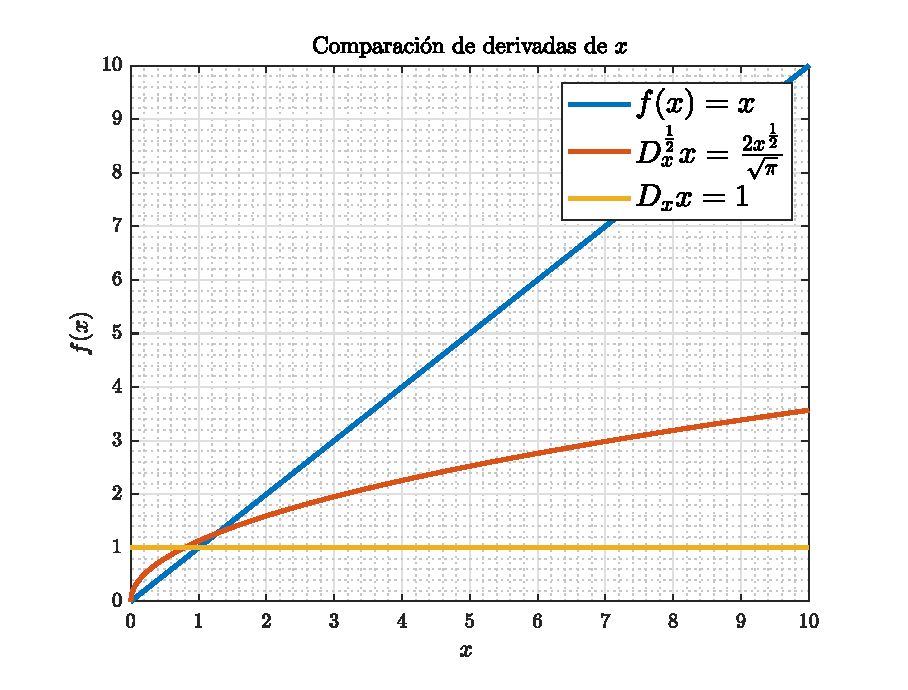
\includegraphics[width = 9cm]{A3_derivada_x.eps}
			\caption{Comparación de derivada entera y fraccionaria.}
		\end{figure}
	\end{frame}	
	
	\begin{frame}
		\frametitle{Introducción}
		\begin{block}{Aplicaciones}
			\begin{itemize}
			\justifying
				\item Describir relación $i$-$v$ en una linea de transmisión.
				\item Representar difusión de calor a través de un solido.
				\item Modelado de sistema metalúrgico industrial.
				\item Mejorar robustez de un control PID para motores DC.
			\end{itemize}
		\end{block}
			
	\end{frame}	
	
	\begin{frame}
		\frametitle{Introducción}
		\begin{block}{Osciladores caóticos y el cálculo fraccionario}
		\justifying
		Oscilador caótico de Chen de orden fraccionario
		\[\left\{ \begin{array}{rl}
		 	_{0} D_{t}^{\,\,q_{1}} x(t)= & a (y(t) - x(t)) \\
		 	&\\
			_{0} D_{t}^{\,\,q_{2}} y(t)= & (c - a) x(t) - x(t) z(t) + cy(t) \\
			&\\
			_{0} D_{t}^{\,\,q_{3}} z(t)= &  x(t) y(t) - b z(t)\\
		\end{array}
		\right. \]
		
		donde $q_{1}, q_{2}, q_{3}$ son ordenes de derivadas. El mínimo orden aceptable es $q > 0.8244$. $a = 35$, $b = 3$, $c = 28$ y $d = -7$. Condiciones iniciales $(x(0), y(0), z(0)) = (-9,-5,14)$.
		\end{block}
	\end{frame}	
	
	
	\begin{frame}
		\frametitle{Introducción}
		\begin{figure}[hbtp]
			\centering
			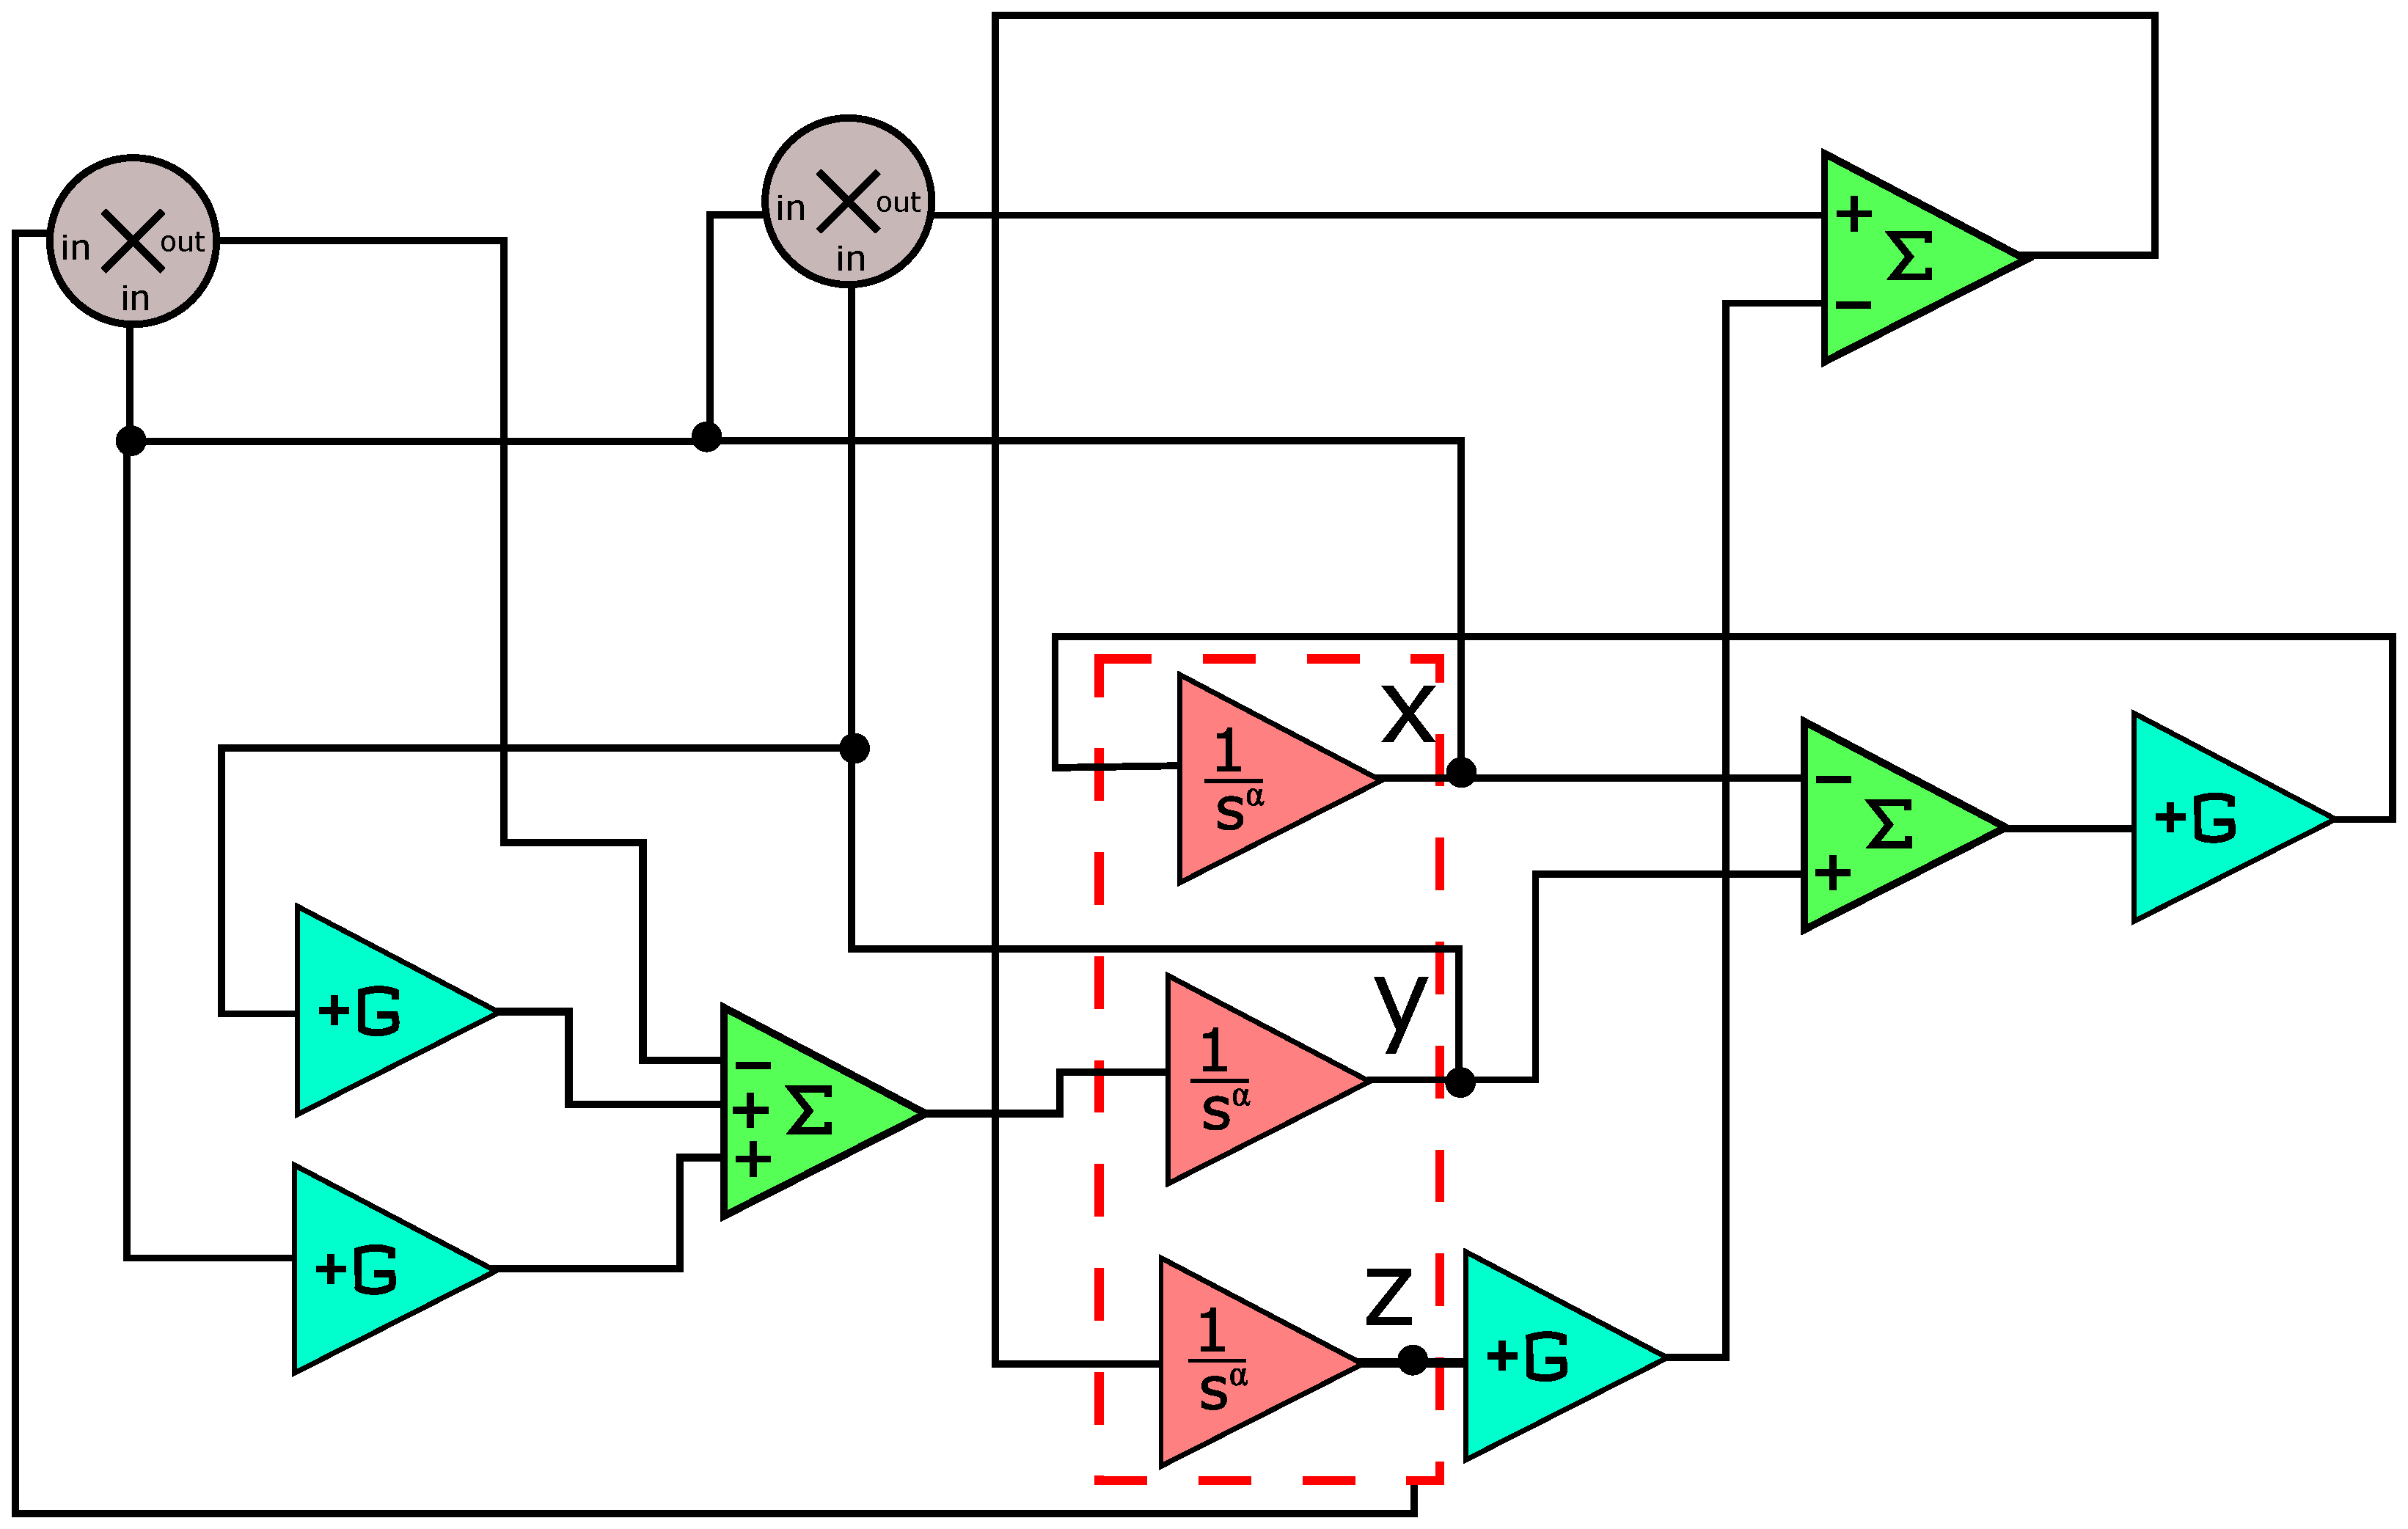
\includegraphics[width = 10cm]{Chen_esquematico.eps}
			\caption{Diagrama a bloques}
		\end{figure}
	\end{frame}
	
	
	\begin{frame}
		\frametitle{Introducción}
		\begin{figure}[hbtp]
			\centering
			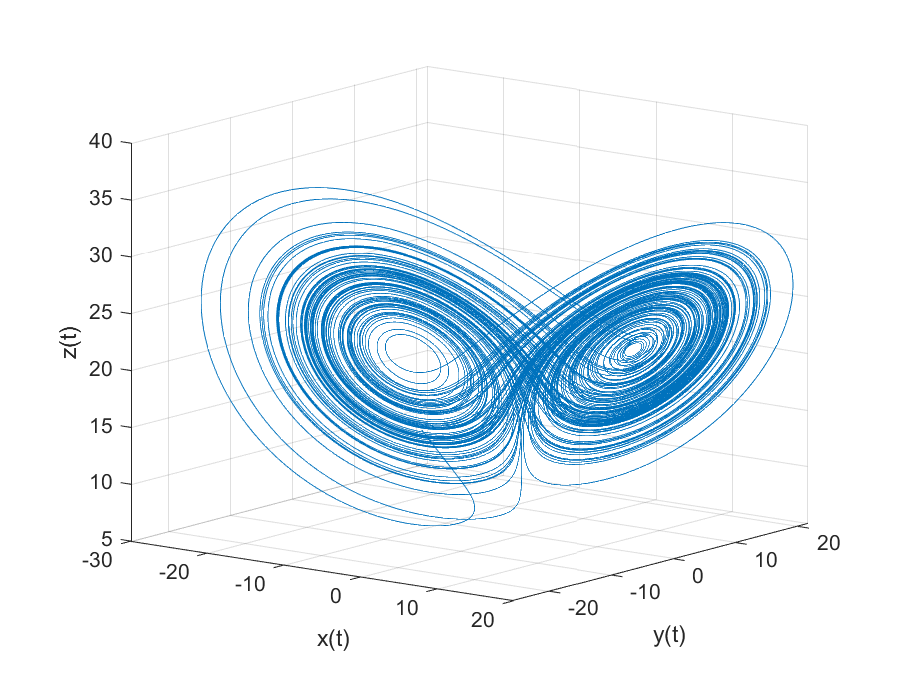
\includegraphics[width = 9cm]{A1_oscilador_de_chen.eps}
			\caption{Atractor de oscilador caótico de Chen de orden fraccionario.}
		\end{figure}
	\end{frame}
	
	\section{Justificación}
	\begin{frame}
		\frametitle{Justificación}
		\begin{block}{Tipos de implementaciones}
		\begin{itemize}
			\item Aplicaciones en aumento.
			\item Necesidad de implementación física.
		\end{itemize}
			\begin{figure}[hbtp]
			\centering
			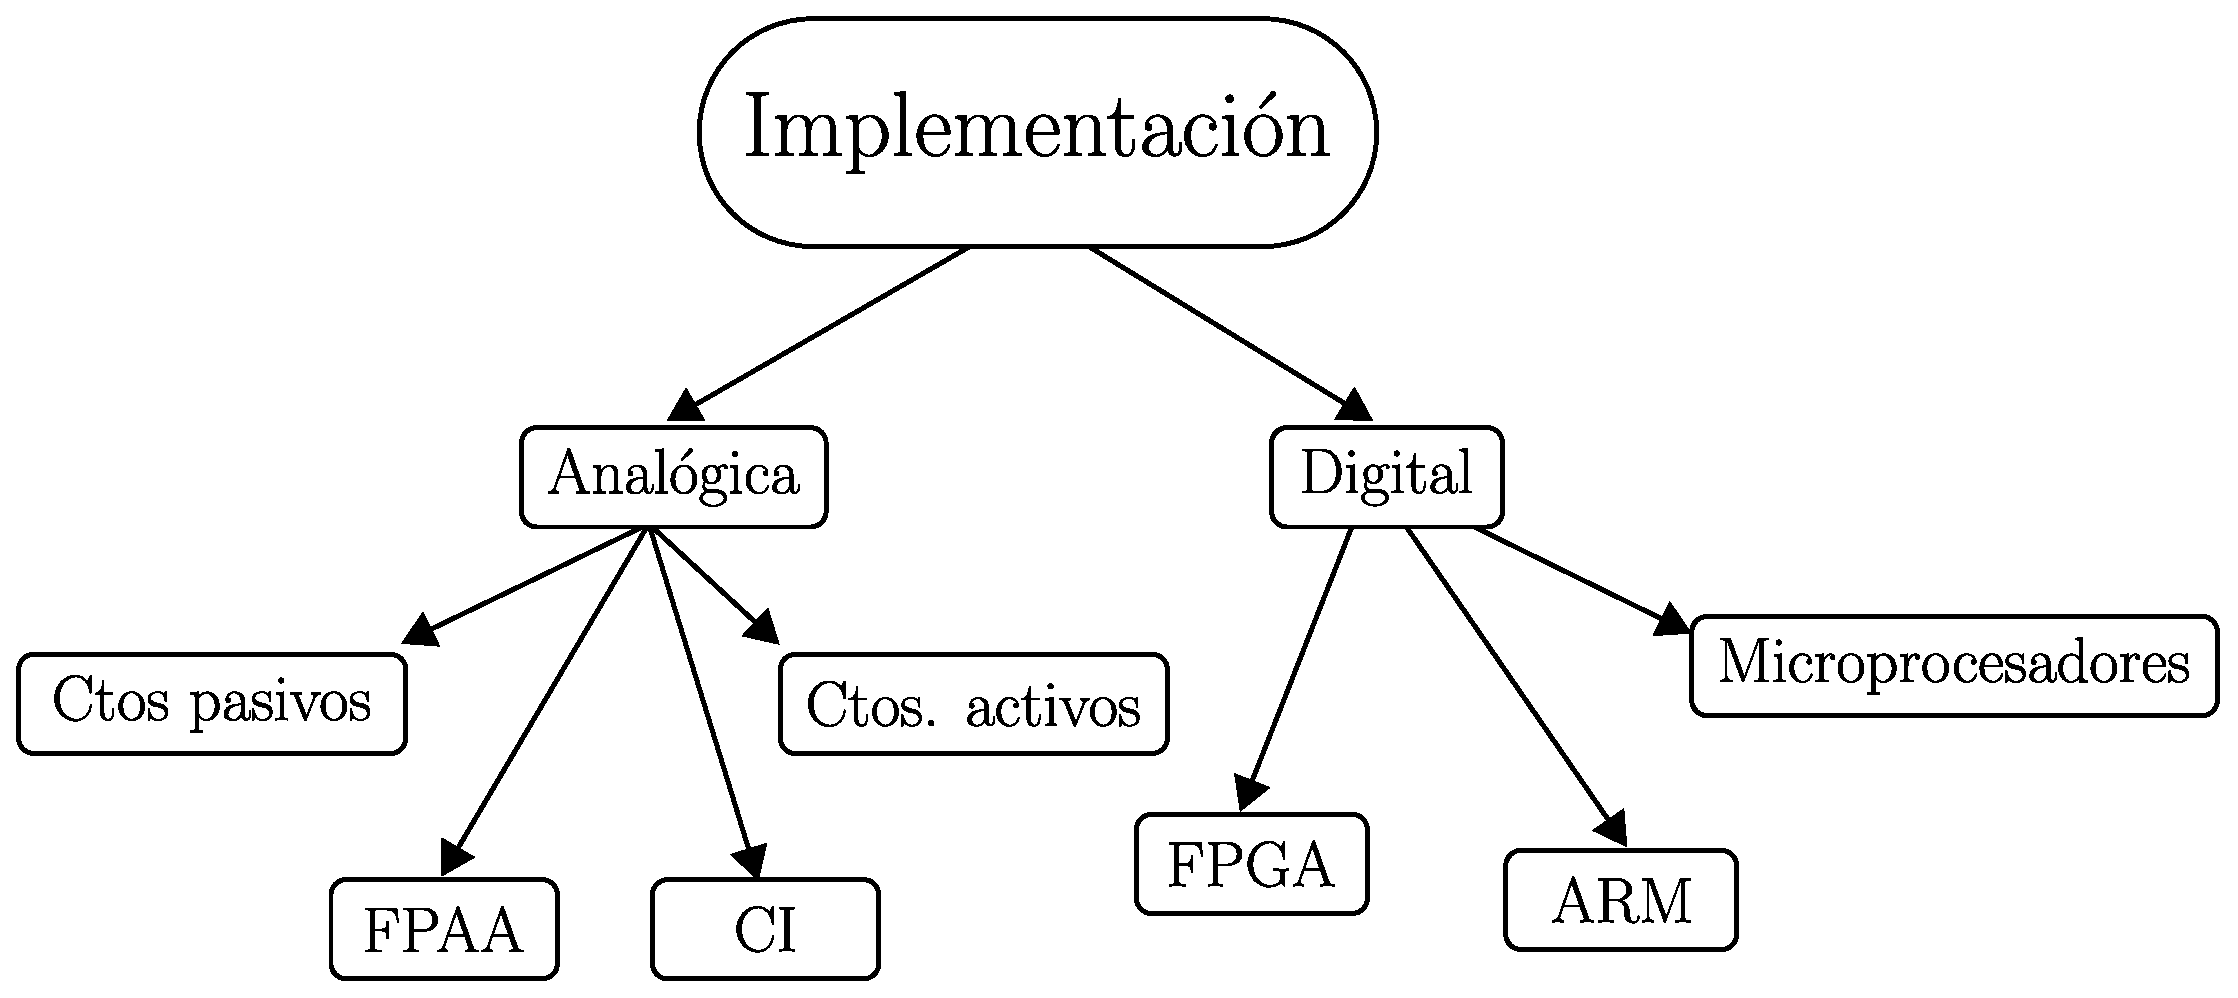
\includegraphics[width = 10cm]{A4_implementacion.eps}
%			\caption{Atractor de oscilador caótico de Chen de orden fraccionario.}
		\end{figure}
		\end{block}
	\end{frame}
	
	
	\begin{frame}
		\frametitle{Justificación}
		\begin{block}{FPAA}
			\begin{itemize}
				\item Versatilidad y facilidad.
				\item FPAA $\to$ Field Programable Analog Array
				\item CAM $\to$ Configurable Analog Modules
				\begin{itemize}
					\item Inversores
					\item Multiplicadores
					\item Filtros
					\item Lookup Table
				\end{itemize}
			\end{itemize}
		\end{block}
	\end{frame}	
	
	\begin{frame}
		\frametitle{Justificación}
		\begin{block}{Aproximación de funciones racionales}
			\begin{itemize}
				\item {\color{blue} Oustaloup} \cite{Gunay2017}
				\item  Carlson
				\item Matsuda
				\item {\color{red}Expansión de Fracciones Continuas (CFE)}
				\begin{itemize}
					\item Dominio de la frecuencia
					\item $20\alpha$ dB/década y 90 $\alpha$ deg.
				\end{itemize}
			\end{itemize}
		\end{block}
	\end{frame}
	
	\begin{frame}
		\frametitle{Justificación}
		\begin{block}{Expansión de fracciones continuas (CFE)}
			\begin{equation}
				x = s-1
			\end{equation}
			\begin{equation}
 		(1 + x)^{\alpha} = \cfrac{1}{1 - \cfrac{\alpha x}{1 + \cfrac{\cfrac{1(1 + \alpha)}{1\cdot2}\,x}{1 + \cfrac{\cfrac{1(1 - \alpha)}{2\cdot3}\,x}{1 + \cfrac{\cfrac{2(2 + \alpha)}{3\cdot4}\,x}{1 + \cfrac{\cfrac{2(2 - k)}{4\cdot5}\,x}{1 + \cfrac{\cfrac{3(3 + \alpha)}{5\cdot6}\,x}{1 + \genfrac{}{}{0pt}{0}{}{\ddots}}}}}}}}
		 	\label{ec:lagrange}
			\end{equation}			
		\end{block}
	\end{frame}
	
	\begin{frame}
		\frametitle{Justificación}
		\begin{figure}[hbtp]
			\centering
			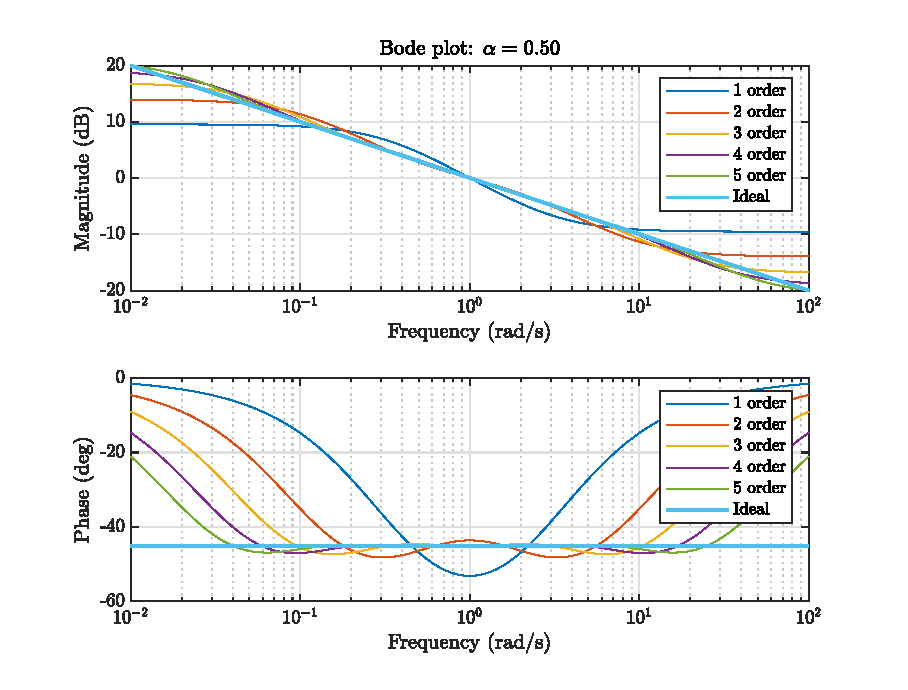
\includegraphics[width = 10cm]{A5_bode.eps}
%			\caption{Atractor de oscilador caótico de Chen de orden fraccionario.}
		\end{figure}
	\end{frame}
	
	\section{Objetivos}
	\begin{frame}
		\frametitle{Objetivos}
		\begin{block}{Objetivo general}
		\justifying
			Diseño e implementación electrónica de integradores de orden fraccionario mediante una expansión de fracciones continuas (CFE) para su aplicación en sistemas caóticos.
		\end{block}
		
		\begin{block}{Objetivos específicos}
			\begin{itemize}
			\justifying
				\item Analizar el método de expansión de fracciones continuas para generar una metodología de diseño en MATLAB.
				\item Caracterizar el error de la expansión de fracciones continuas para generar reglas de diseño.
				\item Diseñar e implementar en FPAA el integrador de orden fraccionario con aproximaciones de ordenes superiores.
				\item Diseñar e implementar de FPAA un oscilador caótico de orden fraccionario	
			\end{itemize}
		\end{block}
	\end{frame}
	
	
	
	\section{Descripción}
	\begin{frame}
		\frametitle{Descripción}
		\begin{figure}[hbtp]
			\centering
			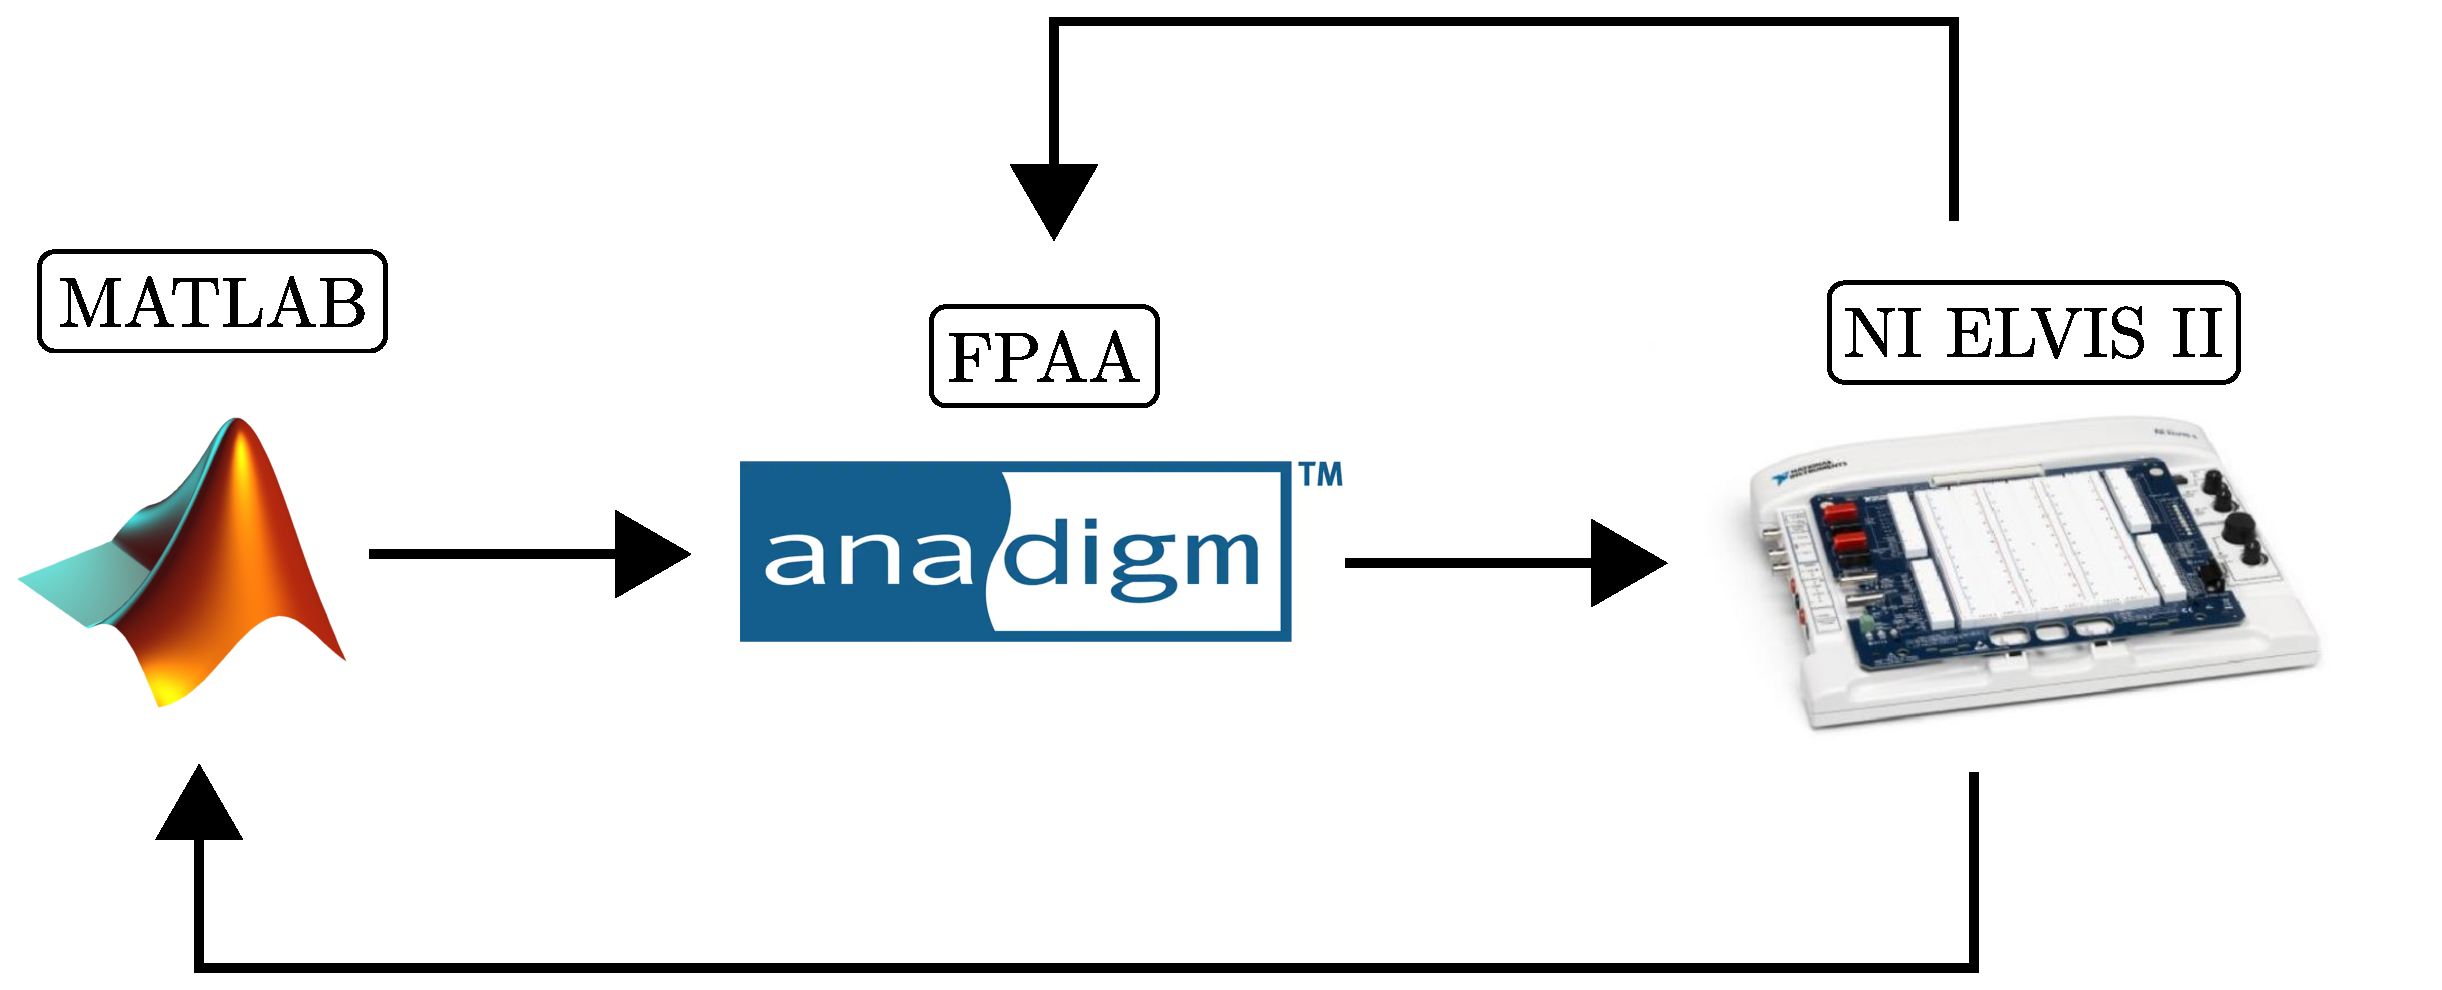
\includegraphics[width = 12cm]{descripcion.eps}
%			\caption{Atractor de oscilador caótico de Chen de orden fraccionario.}
		\end{figure}
	\end{frame}
	
	\section{Diagrama de bloques}
	\begin{frame}
		\frametitle{Diagrama de bloques}
		\begin{figure}[hbtp]
			\centering
			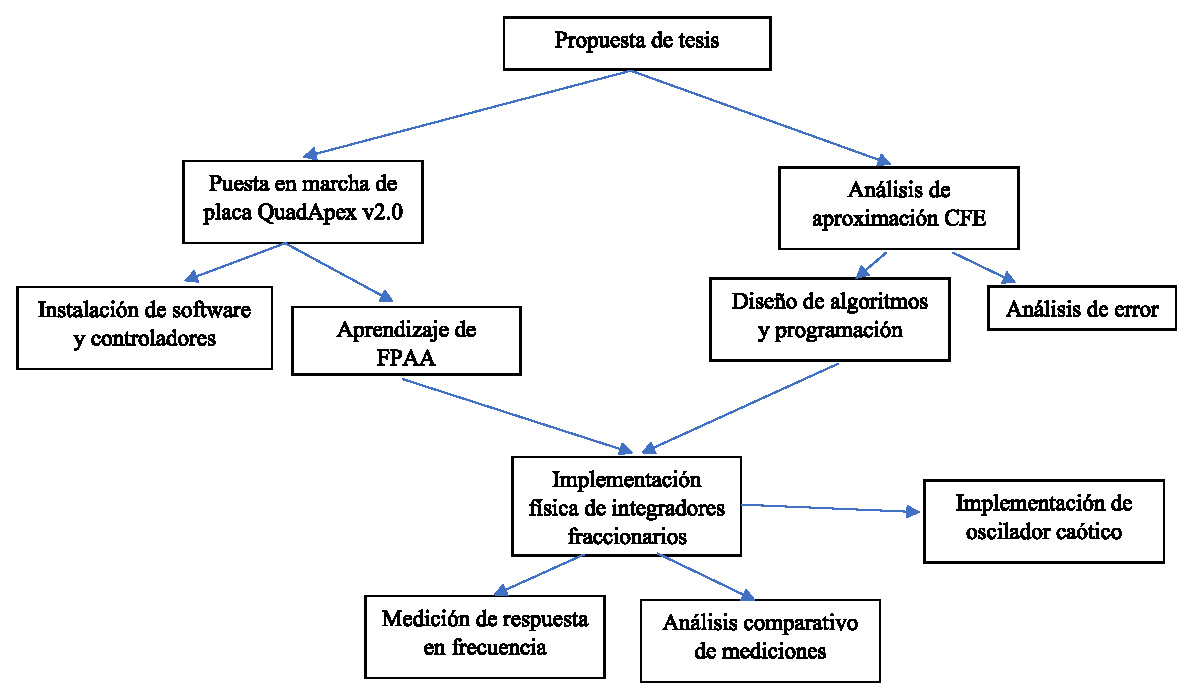
\includegraphics[width = 10cm]{diagrama_de_bloques.eps}
%			\caption{Atractor de oscilador caótico de Chen de orden fraccionario.}
		\end{figure}
	\end{frame}
	
	\section{Cronograma de actividades}
	\begin{frame}
		\frametitle{Cronograma de actividades}
		\begin{figure}[hbtp]
			\centering
			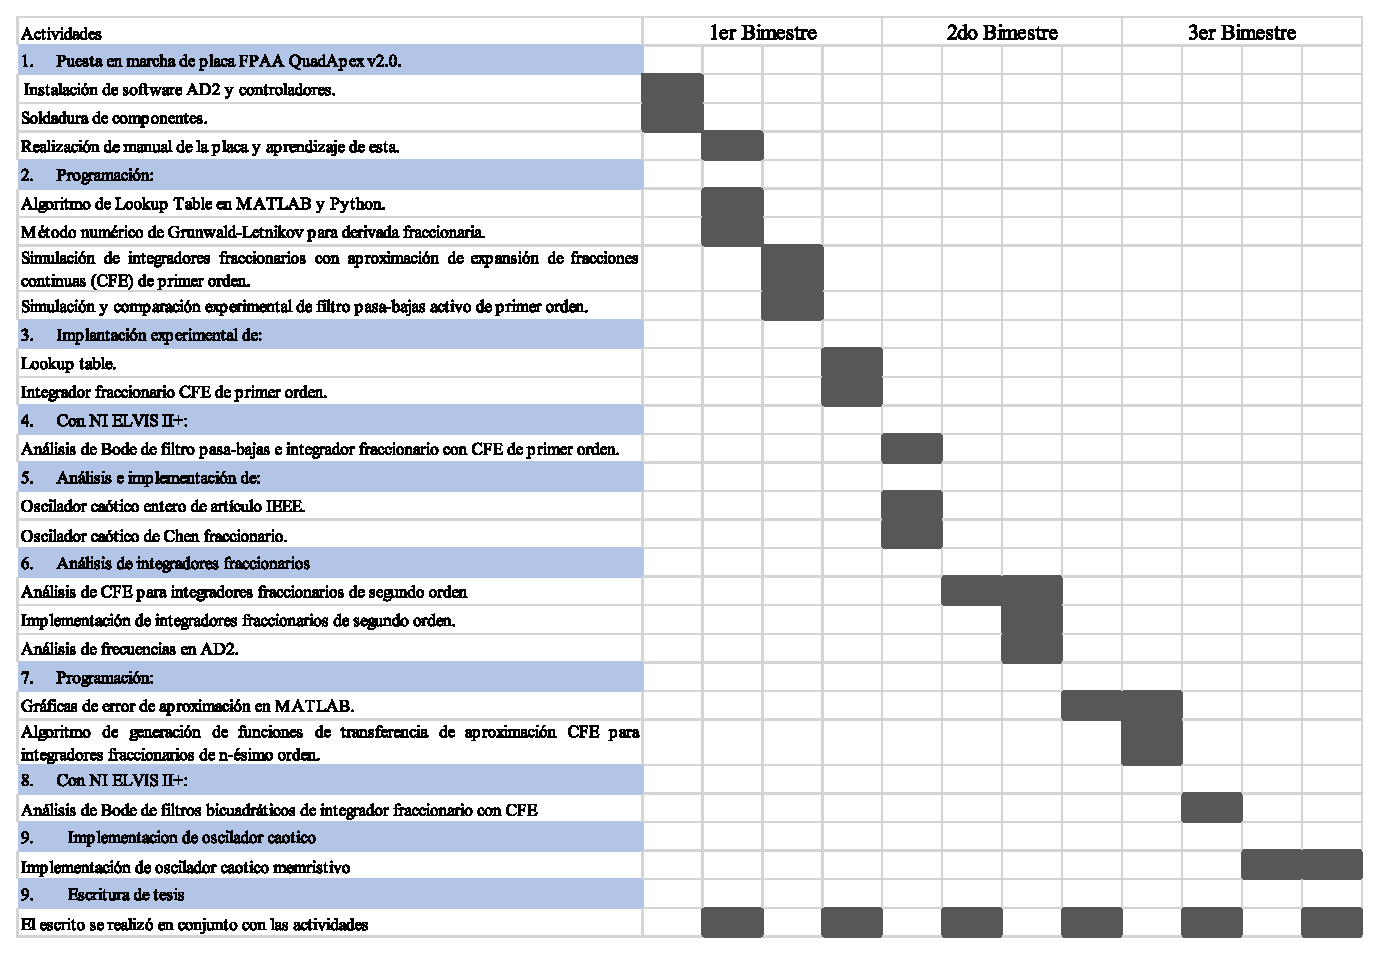
\includegraphics[width = 10cm]{cronograma_de_actividades.eps}
%			\caption{Atractor de oscilador caótico de Chen de orden fraccionario.}
		\end{figure}
	\end{frame}
	
	
	\section{Bibliografía}
	\begin{frame}[t, allowframebreaks]
		\frametitle{Bibliografía}
		\nocite{*}
		\bibliographystyle{ieeetr}
		\bibliography{bibliografia}
	\end{frame}
	
	\begin{frame}
		\frametitle{Introducción}
		\begin{block}{¿Qué es el caos?}
		\justifying
			El caos se refiere a un tipo de comportamiento dinámico complejo que posee algunas características muy especiales:
			\begin{itemize}
				\item Se describe mediante un conjunto de ecuaciones diferenciales ordinarias.
				\item Posee extrema sensibilidad a pequeñas variaciones.
				\item Presenta trayectorias encerradas en el espacio de fase.
			\end{itemize}
		\end{block}
	\end{frame}	
	
	
		\begin{frame}
		\frametitle{Introducción}
		\begin{block}{Aplicaciones de osciladores caóticos}
			\begin{itemize}
				\item Técnicas de modulación.
				\item Sistemas de comunicación.
				\item Encriptación de datos usando caos.
				\item Modelado de sistemas biológicos.
				\item Reacciones químicas.
				\item Toma de decisiones criticas en política, economía y eventos militares.
				\end{itemize}
		\end{block}
		
\begin{figure}[!h]
	\begin{minipage}[c]{0.45\textwidth}
		\centering
		\includegraphics[width = 3.5cm]{encrypt.png}
%		\caption{Oscilador caótico de Chen de orden fraccionario.}
	\end{minipage} \hfill \begin{minipage}[c]{0.45\textwidth}
		\centering
		\includegraphics[width = 4cm]{comunication.png}
%		\caption{Oscilador caótico de Chen de orden fraccionario.}
	\end{minipage}
\end{figure}
	\end{frame}



\end{document}